\section{Plateformes de développement}\label{sec:etat_art-802.15.4}
\renewcommand{\rightmark}{Plateformes de développement}
\subsection*{Zolertia RE-Mote}
Pour ce mémoire, la plateforme Zolertia RE-Mote revision B(Fig.~\ref{fig:state-zolertia}) est utilisée.

Cette plateforme, basée sur un system on chip (SoC) CC2538 ARM Cortex-M3, a été conçue par des universités et des industriels dans le but de permettre aux chercheurs et makers de développer des applications IoT et des objets connectés.

Le Zolertia RE-Mote a été choisi car elle est équipée de deux radios compatibles IEEE 802.15.4,
permet une consommation électrique faible et possède de nombreux pins de connexion qui peuvent être utilisés pour y connecter des capteurs, actuateurs, radios, etc.

Le prix du consturcteur pour cette plateforme est de 93,95€~\cite{zolertia-remote:shop}.

\begin{figure}[H]
    \centering
    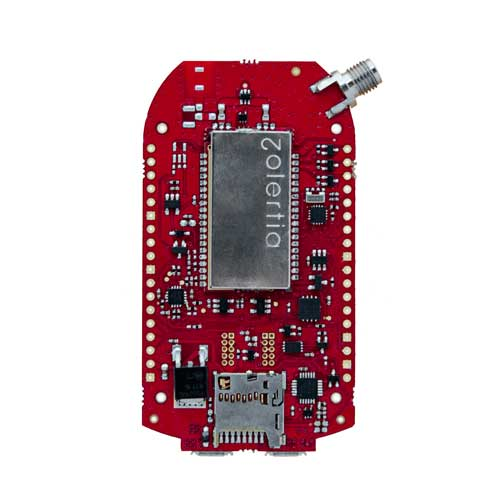
\includegraphics[scale=0.3]{res/remote-zolertia.jpg}
    \caption{Zolertia RE-Mote révision B~\cite{zolertia-remote:shop}.}
    \label{fig:state-zolertia}
\end{figure}

La table~\ref{tb:state-spec} reprend les principales spécifications du Zolertia RE-Mote rev.b et sa table ... la consommation électique.%TODO datasheet ???

\begin{table}[H]
    \centering
    \begin{tabular}{|c|c|}
        \hline
        \rowcolor{lightgray}
        Element            & Spécification\\
        \hline
        Radio              & Deux radios IEEE 802.15.4 à 2.4 GHz et 863-950 MHz\\
        \hline
        CPU                & ARM\textsuperscript{\tiny\textregistered} Cortex\textsuperscript{\tiny\textregistered} -M3 jusqu'à 32 MHz\\
        \hline
        RAM                & 32 KB (16 KB pour tous les Power Modes)\\
        \hline
        Flash programmable & 512KB\\
        \hline
        I/O                & RGB led, boutton user et reset, USB 2.0 à 12Mbps, Real-Time Clock\\
        \hline
    \end{tabular}
    \caption{Spécifications du Zolertia RE-Mote rev.b~\cite{zolertia-remote:datasheet}.}
    \label{tb:state-spec} reprend la consommation de courant du RN2483 
\end{table}

\subsection*{RN2483}
    Le RN2483 (Fig.~\ref{fig:state-rn2483}) est un modem LoRa compatible LoRaWAN$^{TM}$ basse énergie.
    La communication avec ce modem ce fait par des commandes ASCII envoyée via une interface UART. Il prend en charge les modulations FSK, GFSK et LoRa. Il possède également 14 GPIOs ??pour le contrôle et le status, partagés avec 14 inputs analogiques.??%TODO
    Ses fréquences opérationnelles sont situées dans les bandes de fréquences 433 MHz et 868 MHz. D'après la datasheet, 
    sa portée maximale est de 15km en agglomération et 5km en zone urbaine. Comme l'illustre la figure.~\ref{fig:state-rn2483}, pour ce mémoire, le RN2483 a été monté sur un carte d'interface réalisée par B.Quoitin qui comporte deux leds, une petite antenne ainsi que les connecteurs permettant d'utiliser des câbles de prototypages.

    \begin{figure}[H]%TODO changer figure
        \centering
        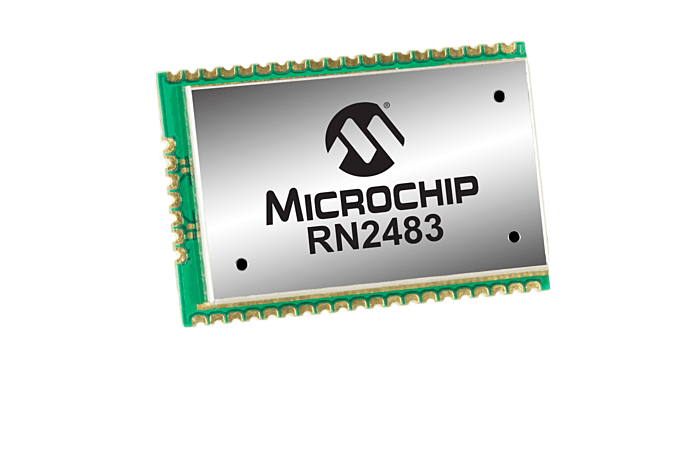
\includegraphics[scale=0.3]{res/rn2483.png}
        \caption{RN2483~\cite{rn2483:shop}.}
        \label{fig:state-rn2483}
    \end{figure}

    La figure \ref{fig:state-rn2484-block} reprend le schéma-bloc du RN2483. Il contient notemment l'interface UART, les antennes 433 MHz et 868Mhz ainsi que les GPIOs et la stack LoRaWan.
    \begin{figure}[H]
        \centering
        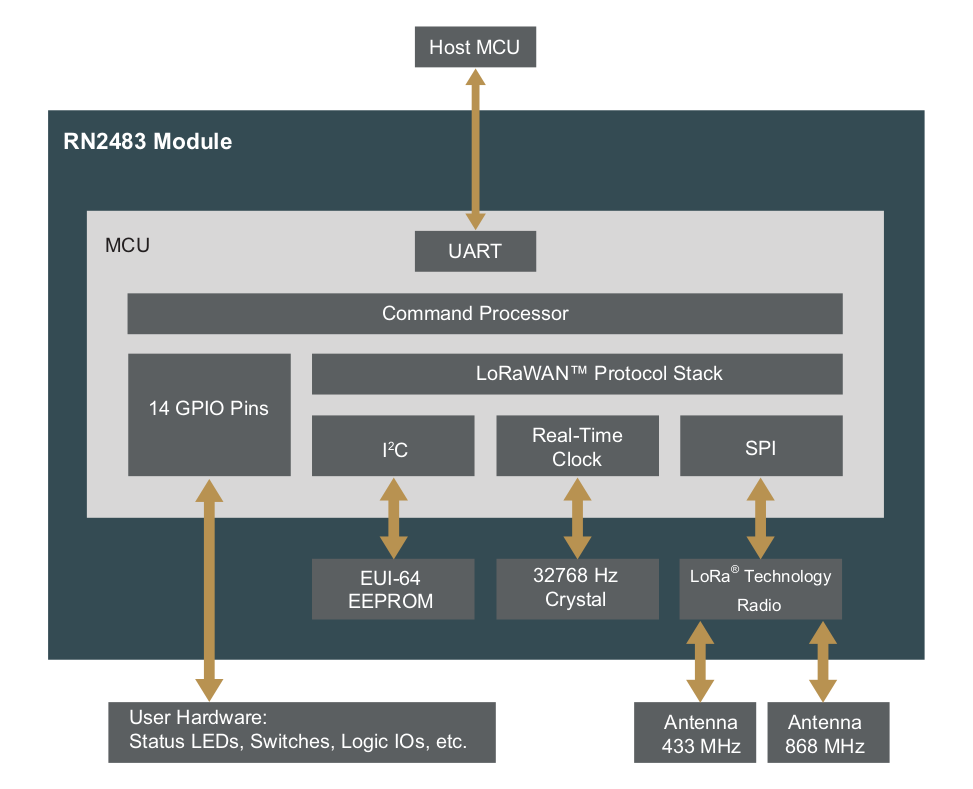
\includegraphics[scale=0.4]{res/rn2483-block-diagram.png}
        \caption{Schéma-bloc du RN2483~\cite{rn2483:datasheet}.}
        \label{fig:state-rn2484-block}
    \end{figure}
    La table~\ref{tb:state-rn2483-consumption} reprend la consommation électrique du RN2483 en fonction de son mode de fonctionnement.
    \begin{table}[H]
        \centering
        \begin{tabular}{| *{4}{c|} }
            \hline
            Mode & \multicolumn{3}{c|}{\multirow{1}{*}{Courant (mA)}}\\ \cline{2-4}
             & VDD = 2.1V & VDD = 3.3V  & VDD = 3.6V \\ \hhline{|=|=|=|=|}
            Idle & 1.7 & 2.8 & 3.1 \\ \hline
            Transmit & 28.6 & 38.9 & 44.5 \\ \hline
            Sleep & 0.0015 & 0.0016 & 0.0016 \\ \hline
            Receive & 12.96 & 14.22 & 14.69 \\ \hline
        \end{tabular}
        \caption{Consommation de courant (à 25 °C) \cite{rn2483:datasheet}.}
        \label{tb:state-rn2483-consumption}
    \end{table}

\subsection*{Raspberry Pi}

Le Raspberri Pi est un ordinateur monocarte. Le modèle utilisé pour ce projet est un Raspberry Pi 3 modèle B+ (Fig.~\ref{fig:state-raspberrypi}). La table \ref{tb:state-raspberrypi-spec} reprend les principales caractéristiques de ce modèle.

\begin{figure}[H]
    \centering
    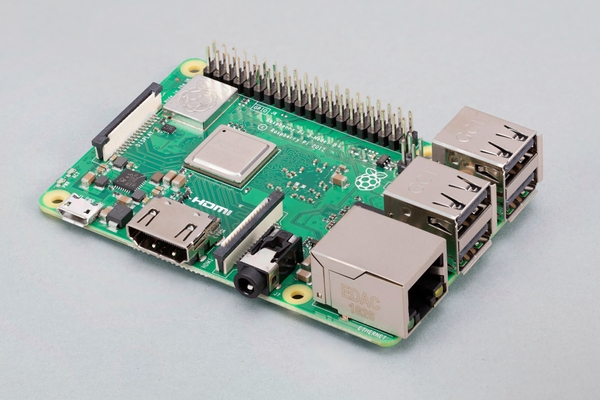
\includegraphics[scale=0.4]{res/raspberrypi3b+.png}
    \caption{Raspberry Pi 3B+~\cite{raspberry:shop}.}
    \label{fig:state-raspberrypi}
\end{figure}

\begin{table}[H]
    \centering
    \begin{tabular}{|c|p{0.75\textwidth}|}
        \hline
        \rowcolor{lightgray}
        Element            & Spécification\\
        CPU & Broadcom BCM2837B0, Cortex-A53 64-bit SoC à 1.4GHz\\ \hline
        Mémoire & 1GB LPDDR2 SDRAM \\ \hline
        Connectivité & 
        \begin{itemize}
            \item IEEE 802.11.b/g/n/ac, Bluetooth 4.2, BLE
            \item Gigabit Ethernet over USB 2.0
            \item 4 × USB 2.0 ports
        \end{itemize}\\ \hline
        Alimentation & 5V/2.5A DC\\ \hline
    \end{tabular}
    \caption{Spécifications du Raspberry Pi 3B+ \cite{raspberry:shop}.}
    \label{tb:state-raspberrypi-spec}
\end{table}
